\begin{pastexam}[label={px:ncku-114-prog-09}]{成大資訊聯招 114 學年度 第 9 題}
（複選；至少有二個正確答案）

{[4\%]} Considering the following two sequences, which are traversal results of a binary tree.
\begin{itemize}
\item Inorder-traversal result: \quad H D I N B E J A O K P F L C G M
\item Postorder-traversal result: \quad H N I D J E B O P K L F M G C A
\end{itemize}
Please reconstruct the binary tree using the above two sequences. Which of the following descriptions are correct for the resultant binary tree?

\textbf{Note: In a tree, each step from top to bottom is called the level of a tree. The level count starts with 1 and increments by 1 at each level or step.}
\begin{enumerate}[label=(\Alph*)]
\item The balance factor of the root is 0.
\item The height of the tree is 4.
\item The total number of leaf nodes is 7.
\item After performing a depth-first search starting at node B of the resultant tree, the shortest path from vertex B to vertex O in the spanning tree has 5 edges.
\item The last element in the result of level-order traversal of the tree is P.
\end{enumerate}
\end{pastexam}

\begin{pastsoln}
答案：(A)、(C)、(D)、(E)。 (B) 照題目「層數從 $1$ 算」的定義，樹高是 $5$，錯；若樹高用邊數算才是 $4$。

\textbf{重建}（資結書第~7.4~節）：後序的最後一個是根；在中序裡找到根，左邊是左子樹、右邊是右子樹；左子樹有幾個節點，
後序前面就取幾個給左子樹，遞迴下去。
\begin{itemize}
\item 後序最後是 A。 中序 \texttt{HDINBEJ | A | OKPFLCGM}：左子樹 $7$ 個，後序切成 \texttt{HNIDJEB} 和 \texttt{OPKLFMGC}。
\item 左子樹：根 B；中序 \texttt{HDIN | B | EJ}。 \texttt{HDIN}（後序 \texttt{HNID}）的根 D，左 H，右 \texttt{IN}（後序
\texttt{NI}）：根 I，N 是 I 的右子節點。 \texttt{EJ}（後序 \texttt{JE}）：根 E，J 是右子節點。
\item 右子樹：根 C；中序 \texttt{OKPFL | C | GM}。 \texttt{OKPFL}（後序 \texttt{OPKLF}）的根 F，左 \texttt{OKP}（後序
\texttt{OPK}）：根 K，左 O、右 P；右 L。 \texttt{GM}（後序 \texttt{MG}）：根 G，M 是右子節點。
\end{itemize}
\begin{center}
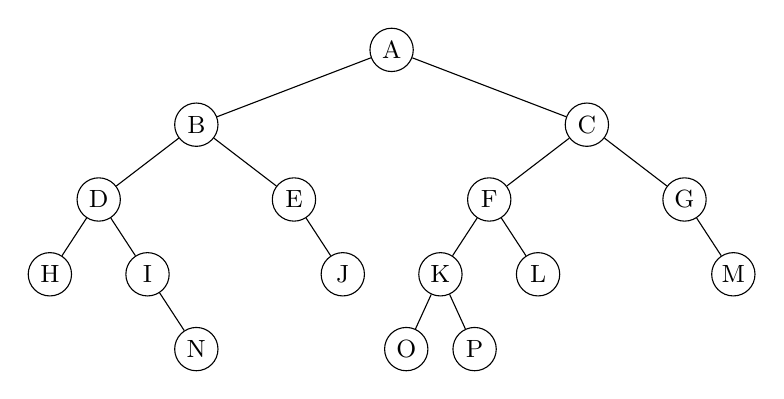
\begin{tikzpicture}[x=0.62cm,y=0.95cm,v/.style={circle,draw,inner sep=0pt,minimum size=5.5mm,font=\small}]
\node[v] (A) at (8,0) {A};
\node[v] (B) at (4,-1) {B}; \node[v] (C) at (12,-1) {C};
\node[v] (D) at (2,-2) {D}; \node[v] (E) at (6,-2) {E}; \node[v] (F) at (10,-2) {F}; \node[v] (G) at (14,-2) {G};
\node[v] (H) at (1,-3) {H}; \node[v] (I) at (3,-3) {I}; \node[v] (J) at (7,-3) {J}; \node[v] (K) at (9,-3) {K}; \node[v] (L) at (11,-3) {L}; \node[v] (M) at (15,-3) {M};
\node[v] (N) at (4,-4) {N}; \node[v] (O) at (8.3,-4) {O}; \node[v] (P) at (9.7,-4) {P};
\draw (A)--(B) (A)--(C) (B)--(D) (B)--(E) (C)--(F) (C)--(G) (D)--(H) (D)--(I) (E)--(J) (F)--(K) (F)--(L) (G)--(M) (I)--(N) (K)--(O) (K)--(P);
\end{tikzpicture}
\end{center}
核對：這棵樹的中序是 \texttt{HDINBEJAOKPFLCGM}、後序是 \texttt{HNIDJEBOPKLFMGCA}，和題目相同。

逐項檢查：
\begin{itemize}
\item (A) 對。 根 A 的左子樹（以 B 為根）最深到 N（B--D--I--N，$4$ 層），右子樹 C 最深到 O、P（C--F--K--O，$4$ 層），平衡因子 $4 - 4 = 0$。
\item (B) 錯。 最深的節點 N、O、P 在第 $5$ 層，照題目的層數定義樹高是 $5$。 （若把樹高定義成根到最深葉子的邊數，就是 $4$；題目
特別註明層數從 $1$ 算，應以 $5$ 為準。）
\item (C) 對。 葉子是 H、N、J、O、P、L、M，共 $7$ 個。
\item (D) 對。 樹本身就是連通、無環的圖，從 B 做 DFS 得到的生成樹就是這棵樹（每條邊都是樹邊），B 到 O 的路徑唯一：
B--A--C--F--K--O，共 $5$ 條邊。
\item (E) 對。 層序是 \texttt{A; B C; D E F G; H I J K L M; N O P}，最後一個是 P。
\end{itemize}
\end{pastsoln}
